\documentclass[]{krantz}
\usepackage{lmodern}
\usepackage{amssymb,amsmath}
\usepackage{ifxetex,ifluatex}
\usepackage{fixltx2e} % provides \textsubscript
\ifnum 0\ifxetex 1\fi\ifluatex 1\fi=0 % if pdftex
  \usepackage[T1]{fontenc}
  \usepackage[utf8]{inputenc}
\else % if luatex or xelatex
  \ifxetex
    \usepackage{mathspec}
  \else
    \usepackage{fontspec}
  \fi
  \defaultfontfeatures{Ligatures=TeX,Scale=MatchLowercase}
\fi
% use upquote if available, for straight quotes in verbatim environments
\IfFileExists{upquote.sty}{\usepackage{upquote}}{}
% use microtype if available
\IfFileExists{microtype.sty}{%
\usepackage[]{microtype}
\UseMicrotypeSet[protrusion]{basicmath} % disable protrusion for tt fonts
}{}
\PassOptionsToPackage{hyphens}{url} % url is loaded by hyperref
\usepackage[unicode=true]{hyperref}
\PassOptionsToPackage{usenames,dvipsnames}{color} % color is loaded by hyperref
\hypersetup{
            pdftitle={Limitations of Interpretable Machine Learning Methods},
            colorlinks=true,
            linkcolor=Maroon,
            citecolor=Blue,
            urlcolor=Blue,
            breaklinks=true}
\urlstyle{same}  % don't use monospace font for urls
\usepackage{natbib}
\bibliographystyle{apalike}
\usepackage{color}
\usepackage{fancyvrb}
\newcommand{\VerbBar}{|}
\newcommand{\VERB}{\Verb[commandchars=\\\{\}]}
\DefineVerbatimEnvironment{Highlighting}{Verbatim}{commandchars=\\\{\}}
% Add ',fontsize=\small' for more characters per line
\usepackage{framed}
\definecolor{shadecolor}{RGB}{248,248,248}
\newenvironment{Shaded}{\begin{snugshade}}{\end{snugshade}}
\newcommand{\KeywordTok}[1]{\textcolor[rgb]{0.13,0.29,0.53}{\textbf{#1}}}
\newcommand{\DataTypeTok}[1]{\textcolor[rgb]{0.13,0.29,0.53}{#1}}
\newcommand{\DecValTok}[1]{\textcolor[rgb]{0.00,0.00,0.81}{#1}}
\newcommand{\BaseNTok}[1]{\textcolor[rgb]{0.00,0.00,0.81}{#1}}
\newcommand{\FloatTok}[1]{\textcolor[rgb]{0.00,0.00,0.81}{#1}}
\newcommand{\ConstantTok}[1]{\textcolor[rgb]{0.00,0.00,0.00}{#1}}
\newcommand{\CharTok}[1]{\textcolor[rgb]{0.31,0.60,0.02}{#1}}
\newcommand{\SpecialCharTok}[1]{\textcolor[rgb]{0.00,0.00,0.00}{#1}}
\newcommand{\StringTok}[1]{\textcolor[rgb]{0.31,0.60,0.02}{#1}}
\newcommand{\VerbatimStringTok}[1]{\textcolor[rgb]{0.31,0.60,0.02}{#1}}
\newcommand{\SpecialStringTok}[1]{\textcolor[rgb]{0.31,0.60,0.02}{#1}}
\newcommand{\ImportTok}[1]{#1}
\newcommand{\CommentTok}[1]{\textcolor[rgb]{0.56,0.35,0.01}{\textit{#1}}}
\newcommand{\DocumentationTok}[1]{\textcolor[rgb]{0.56,0.35,0.01}{\textbf{\textit{#1}}}}
\newcommand{\AnnotationTok}[1]{\textcolor[rgb]{0.56,0.35,0.01}{\textbf{\textit{#1}}}}
\newcommand{\CommentVarTok}[1]{\textcolor[rgb]{0.56,0.35,0.01}{\textbf{\textit{#1}}}}
\newcommand{\OtherTok}[1]{\textcolor[rgb]{0.56,0.35,0.01}{#1}}
\newcommand{\FunctionTok}[1]{\textcolor[rgb]{0.00,0.00,0.00}{#1}}
\newcommand{\VariableTok}[1]{\textcolor[rgb]{0.00,0.00,0.00}{#1}}
\newcommand{\ControlFlowTok}[1]{\textcolor[rgb]{0.13,0.29,0.53}{\textbf{#1}}}
\newcommand{\OperatorTok}[1]{\textcolor[rgb]{0.81,0.36,0.00}{\textbf{#1}}}
\newcommand{\BuiltInTok}[1]{#1}
\newcommand{\ExtensionTok}[1]{#1}
\newcommand{\PreprocessorTok}[1]{\textcolor[rgb]{0.56,0.35,0.01}{\textit{#1}}}
\newcommand{\AttributeTok}[1]{\textcolor[rgb]{0.77,0.63,0.00}{#1}}
\newcommand{\RegionMarkerTok}[1]{#1}
\newcommand{\InformationTok}[1]{\textcolor[rgb]{0.56,0.35,0.01}{\textbf{\textit{#1}}}}
\newcommand{\WarningTok}[1]{\textcolor[rgb]{0.56,0.35,0.01}{\textbf{\textit{#1}}}}
\newcommand{\AlertTok}[1]{\textcolor[rgb]{0.94,0.16,0.16}{#1}}
\newcommand{\ErrorTok}[1]{\textcolor[rgb]{0.64,0.00,0.00}{\textbf{#1}}}
\newcommand{\NormalTok}[1]{#1}
\usepackage{longtable,booktabs}
% Fix footnotes in tables (requires footnote package)
\IfFileExists{footnote.sty}{\usepackage{footnote}\makesavenoteenv{long table}}{}
\usepackage{graphicx,grffile}
\makeatletter
\def\maxwidth{\ifdim\Gin@nat@width>\linewidth\linewidth\else\Gin@nat@width\fi}
\def\maxheight{\ifdim\Gin@nat@height>\textheight\textheight\else\Gin@nat@height\fi}
\makeatother
% Scale images if necessary, so that they will not overflow the page
% margins by default, and it is still possible to overwrite the defaults
% using explicit options in \includegraphics[width, height, ...]{}
\setkeys{Gin}{width=\maxwidth,height=\maxheight,keepaspectratio}
\IfFileExists{parskip.sty}{%
\usepackage{parskip}
}{% else
\setlength{\parindent}{0pt}
\setlength{\parskip}{6pt plus 2pt minus 1pt}
}
\setlength{\emergencystretch}{3em}  % prevent overfull lines
\providecommand{\tightlist}{%
  \setlength{\itemsep}{0pt}\setlength{\parskip}{0pt}}
\setcounter{secnumdepth}{5}
% Redefines (sub)paragraphs to behave more like sections
\ifx\paragraph\undefined\else
\let\oldparagraph\paragraph
\renewcommand{\paragraph}[1]{\oldparagraph{#1}\mbox{}}
\fi
\ifx\subparagraph\undefined\else
\let\oldsubparagraph\subparagraph
\renewcommand{\subparagraph}[1]{\oldsubparagraph{#1}\mbox{}}
\fi

% set default figure placement to htbp
\makeatletter
\def\fps@figure{htbp}
\makeatother

\usepackage{booktabs}
\usepackage{longtable}
\usepackage[bf,singlelinecheck=off]{caption}

\usepackage{framed,color}
\definecolor{shadecolor}{RGB}{248,248,248}

\renewcommand{\textfraction}{0.05}
\renewcommand{\topfraction}{0.8}
\renewcommand{\bottomfraction}{0.8}
\renewcommand{\floatpagefraction}{0.75}

\renewenvironment{quote}{\begin{VF}}{\end{VF}}
\let\oldhref\href
\renewcommand{\href}[2]{#2\footnote{\url{#1}}}

\makeatletter
\newenvironment{kframe}{%
\medskip{}
\setlength{\fboxsep}{.8em}
 \def\at@end@of@kframe{}%
 \ifinner\ifhmode%
  \def\at@end@of@kframe{\end{minipage}}%
  \begin{minipage}{\columnwidth}%
 \fi\fi%
 \def\FrameCommand##1{\hskip\@totalleftmargin \hskip-\fboxsep
 \colorbox{shadecolor}{##1}\hskip-\fboxsep
     % There is no \\@totalrightmargin, so:
     \hskip-\linewidth \hskip-\@totalleftmargin \hskip\columnwidth}%
 \MakeFramed {\advance\hsize-\width
   \@totalleftmargin\z@ \linewidth\hsize
   \@setminipage}}%
 {\par\unskip\endMakeFramed%
 \at@end@of@kframe}
\makeatother

\renewenvironment{Shaded}{\begin{kframe}}{\end{kframe}}

\usepackage{makeidx}
\makeindex

\urlstyle{tt}

\usepackage{amsthm}
\makeatletter
\def\thm@space@setup{%
  \thm@preskip=8pt plus 2pt minus 4pt
  \thm@postskip=\thm@preskip
}
\makeatother

\frontmatter

\title{Limitations of Interpretable Machine Learning Methods}
\date{2019-05-21}

\begin{document}
\maketitle

% you may need to leave a few empty pages before the dedication page

%\cleardoublepage\newpage\thispagestyle{empty}\null
%\cleardoublepage\newpage\thispagestyle{empty}\null
%\cleardoublepage\newpage
\thispagestyle{empty}

\begin{center}
\end{center}

\setlength{\abovedisplayskip}{-5pt}
\setlength{\abovedisplayshortskip}{-5pt}

{
\hypersetup{linkcolor=black}
\setcounter{tocdepth}{2}
\tableofcontents
}
\listoftables
\listoffigures
\chapter*{Preface}\label{preface}


This project explains the limitations of current approaches in
interpretable machine learning, such as partial dependence plots (PDP,
Accumulated Local Effects (ALE), permutation feature importance,
leave-one-covariate out (LOCO) and local interpretable model-agnostic
explanations (LIME). All of those methods can be used to explain the
behavior and predictions of trained machine learning models. The
interpretation methods might not work well in the following cases:

\begin{itemize}
\tightlist
\item
  if a model models interactions (e.g.~when a random forest is used)
\item
  if features strongly correlate with each other
\item
  if the model does not correctly model causal relationships
\item
  if parameters of the interpretation method are not set correctly
\end{itemize}

\section*{Structure of the book}\label{structure-of-the-book}


TODO

\mainmatter

\chapter{Introduction}\label{introduction}

Here is some text

\section{This is a smaller title}\label{this-is-a-smaller-title}

We have a nice figure in Figure \ref{fig:hello}, and also a table in
Table \ref{tab:iris}.

\begin{Shaded}
\begin{Highlighting}[]
\KeywordTok{par}\NormalTok{(}\DataTypeTok{mar =} \KeywordTok{c}\NormalTok{(}\DecValTok{4}\NormalTok{, }\DecValTok{4}\NormalTok{, }\DecValTok{1}\NormalTok{, .}\DecValTok{1}\NormalTok{))}
\KeywordTok{plot}\NormalTok{(cars, }\DataTypeTok{pch =} \DecValTok{19}\NormalTok{)}
\end{Highlighting}
\end{Shaded}

\begin{figure}
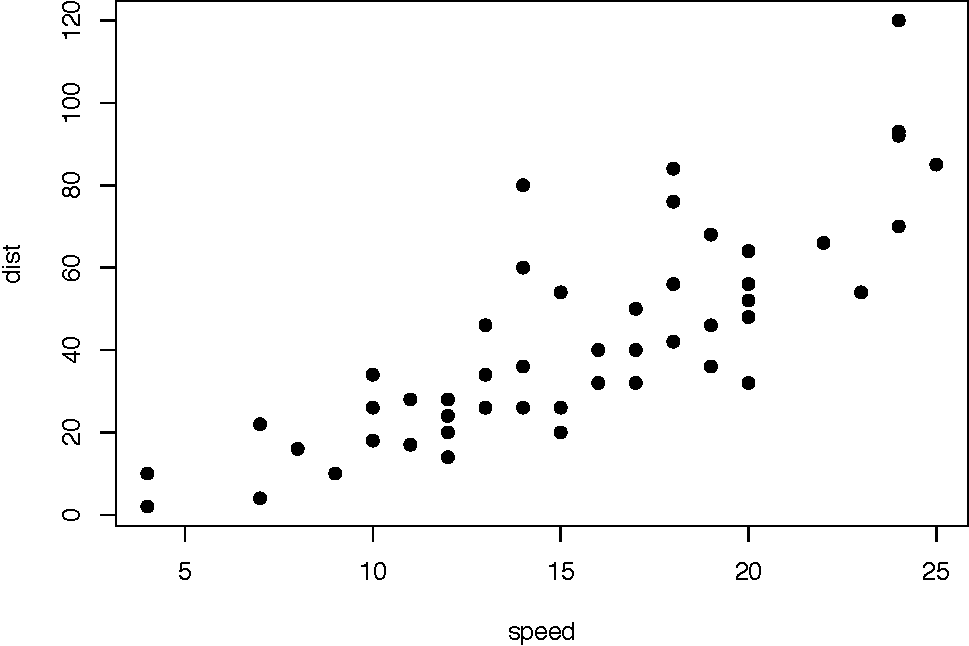
\includegraphics[width=0.9\linewidth]{book_files/figure-latex/hello-1} \caption{Hello World!}\label{fig:hello}
\end{figure}

\begin{Shaded}
\begin{Highlighting}[]
\NormalTok{knitr}\OperatorTok{::}\KeywordTok{kable}\NormalTok{(}
  \KeywordTok{head}\NormalTok{(iris), }\DataTypeTok{caption =} \StringTok{'The boring iris data.'}\NormalTok{,}
  \DataTypeTok{booktabs =} \OtherTok{TRUE}
\NormalTok{)}
\end{Highlighting}
\end{Shaded}

\begin{table}[t]

\caption{\label{tab:iris}The boring iris data.}
\centering
\begin{tabular}{rrrrl}
\toprule
Sepal.Length & Sepal.Width & Petal.Length & Petal.Width & Species\\
\midrule
5.1 & 3.5 & 1.4 & 0.2 & setosa\\
4.9 & 3.0 & 1.4 & 0.2 & setosa\\
4.7 & 3.2 & 1.3 & 0.2 & setosa\\
4.6 & 3.1 & 1.5 & 0.2 & setosa\\
5.0 & 3.6 & 1.4 & 0.2 & setosa\\
\addlinespace
5.4 & 3.9 & 1.7 & 0.4 & setosa\\
\bottomrule
\end{tabular}
\end{table}

\chapter{Partial Dependence Plots (PDP) and Individual Conditional
Expectation
Curves}\label{partial-dependence-plots-pdp-and-individual-conditional-expectation-curves}

\section{Partial Dependence Plots}\label{partial-dependence-plots}

\section{ICE}\label{ice}

\chapter{Accumulated Local Effects
(ALE)}\label{accumulated-local-effects-ale}

\section{Motivation}\label{motivation}

As seen in section 2 PDPs don't work well as soon as two or more
features are correlated. This gives rise to the definition of ALEs.
Although their definition makes sense for high dimensional feature
spaces including categorical features, within this section we only treat
a space with two continous features.

\section{The Theoretical Formula}\label{the-theoretical-formula}

The uncentered ALE with respect to a starting point \(z_{0, j}\) is
defined as
\[  \widetilde{ALE}_{\hat{f},~j}(x) = \hat{f}_{x_j,ALE}(x) = \int_{z_{0,~j}}^{x} E_{X_c \mid X_j} [\hat{f}^j(X_j,~X_c)\mid X_j = z_j]~dz_j,\]
where \(\hat{f}\) is an arbitrary prediction function on the
featurespace \(X = (X_j,X_c)\) (with feature of interest \(X_j\) and
other features \(X_c\)) as well as its j-th partial derivative
\(\hat{f}^j(*,*)\).

\subsection{Centering}\label{centering}

The ALE (centered ALE) is defined as

\[  ALE_{\hat{f},~j}(x) = \widetilde{ALE}_{\hat{f},~j}(x) - E_{X_j}[\widetilde{ALE}_{\hat{f},~j}(X_j)]\]

TODO: where do we explain why we center and interpret the centering?

\section{Estimation Formula}\label{estimation-formula}

Since this theoretical formula of no use for a blackbox model with
unknown or even non existing gradients, an approximative approach will
be used. The uncentered ALE can be approximated by the formula

\[ \widehat{\widetilde{ALE}_{\hat{f},j}}(x) = \int_{z_{0,j}}^{x} \sum_{k=1}^{K}   1_{]z_{k-1,~j},~z_{k,~j}]}(x_j) ~ \frac{1}{n_j(k)}\sum_{i:x_j^{(i)}\in N_j(k)} \frac{[\hat{f}(z_{k,j}, x_{\setminus j}^{(i)})-\hat{f}(z_{k-1,j}, x_{\setminus j}^{(i)})]}{z_{k,~j}-z_{k-1,~j}}~dx_j~.  \]

In a first step the relevant dimension of the feature space is divided
into K intervals beginning with the starting point \(z_{0, j}\). As it
is not clear how to exactly divide the feature space, section 3.x deals
with that question. The upper border of the k-th interval is denoted by
\(z_{k, ~j}\) as well as the lower border by \(z_{k-1, ~j}\). \(N_j(k)\)
denotes the k-th interval and \(n_j(k)\) the total number of
observations having the j-value within this interval. \(x_j^{(i)}\) is
the j-value of the i-th observation and correspondingly
\(x_{\setminus j}^{(i)}\) the values of the other features. The term on
the right approximates the expected partial derivative within each
interval. Therefore each instance within an interval is shifted to the
upper and lower bounds of the interval and the total difference of the
prediction is calculated. Devided by the length of the interval this is
a reasonable approximation for the ``local'' effect on the prediction if
the feature of interest changes (cet. par.). By averaging these
approximations over all observations within the k-th interval, we
recieve a rough estimator for the term
\(E_{X_c \mid X_j} [\hat{f}^j(X_j,~X_c)\mid X_j \in N_j(k)]\), which we
take as constant effect for the k-th interval. By integrating over this
step function which represents the locally estimated derivatives, the
(local) changes are accumulated. Thats why the name Accumulated Local
Effects is quite reasonable. This leads directly to the following
approximative formula for the centered ALE
\[   \widehat{ALE_{\hat{f},~j}}(x) = \widehat{\widetilde{ALE}_{\hat{f},~j}}(x) - \frac{1}{n} \sum_{i=1}^{n} \widehat{\widetilde{ALE}_{\hat{f},~j}}(x_j^{(i)})~. 
 \]

\subsection{Implementation Formula}\label{implementation-formula}

As both the centered and the uncentered ALE estimations are piecewise
linear functions (integration over a step function), one can first
calculate the ALE at the interval boundaries and interpolate in a second
step. Therefore the folowing formula proposed by Apley with slightly
changed notation will be useful:

\[  \widehat{\widetilde{ALE}}_{steps, \hat{f},j}(x) =  \sum_{k=1}^{k(x)}   \frac{1}{n_j(k)}\sum_{i:x_j^{(i)}\in N_j(k)} [\hat{f}(z_{k,j}, x_{\setminus j}^{(i)})-\hat{f}(z_{k-1,j}, x_{\setminus j}^{(i)})].  \]
This formula also returns a step function, but the values in each
interval are the accumulated values of the averaged total differences in
each interval.

Two sentences: To transfer this formula to the correct estimator of the
uncentered ALE one has to linearely interpolate the beginning of each
interval with the last value of this estimation formula in this
interval. So to start it one connects the point \((0,z_{0, j})\) with
\((\widehat{\widetilde{ALE}}_{steps, \hat{f},j}(z_{0, j}), z_{1, j})\)
and this point with
\((\widehat{\widetilde{ALE}}_{steps, \hat{f},j}(z_{2, j}), z_{2, j})\)
and so on.

Alternative more mathematically: To transfer this formula into the
correct estimator of the uncentered ALE one has to linearely interpolate
the points
\((\widehat{\widetilde{ALE}}_{steps, \hat{f},j}(z_{k-1, j}), z_{k-1, j})\)
with
\((\widehat{\widetilde{ALE}}_{steps, \hat{f},j}(z_{k, j}), z_{k, j})\)
for \(k \in \{1, ..., K \}\) and
\(\widehat{\widetilde{ALE}}_{steps, \hat{f},j}(z_{0, j}) = 0\).

Since in this formula there is no integral, it is easier to implement.

\section{Intuition and
Interpretation}\label{intuition-and-interpretation}

As the former sections introduced the theoretical basics for the ALE,
this section shall provide the reader with an intuition as well for the
calculation method as for the interpretation. As described above, the
local behaviour of the model with respect to the variable of interest is
estimated by moving the existing data points to the boundaries of their
interval and evaluating the total difference of the prediction for the
``new'' datapoints. Figure 2.1 gives a good intuition for this
procedure.

\begin{figure}
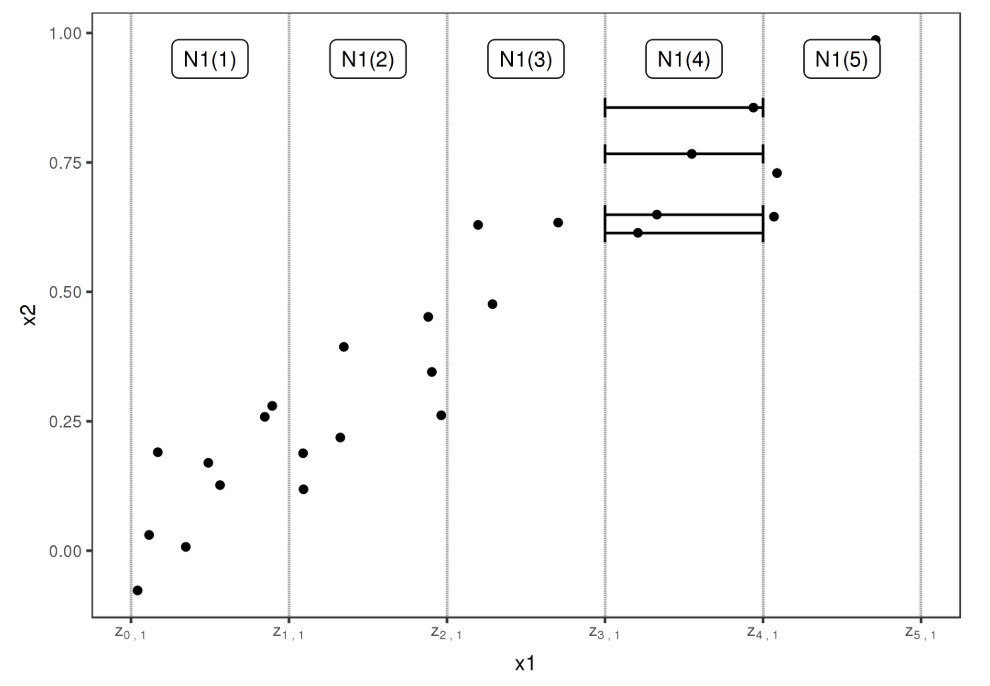
\includegraphics[width=13.75in]{images/ale_estimation_intuition} \caption{bla bla total differences}\label{fig:unnamed-chunk-1}
\end{figure}



TODO: explain it

As the evaluation is done on relatively small intervals, on the one hand
the local behaviour of the model is estimated. On the other hand the
covariance structure of the features is taken into account, as only
``realistic'' datapoints are simulated.

For figure (TODO: reference) 2.1 an ALE could look like this:

\begin{figure}
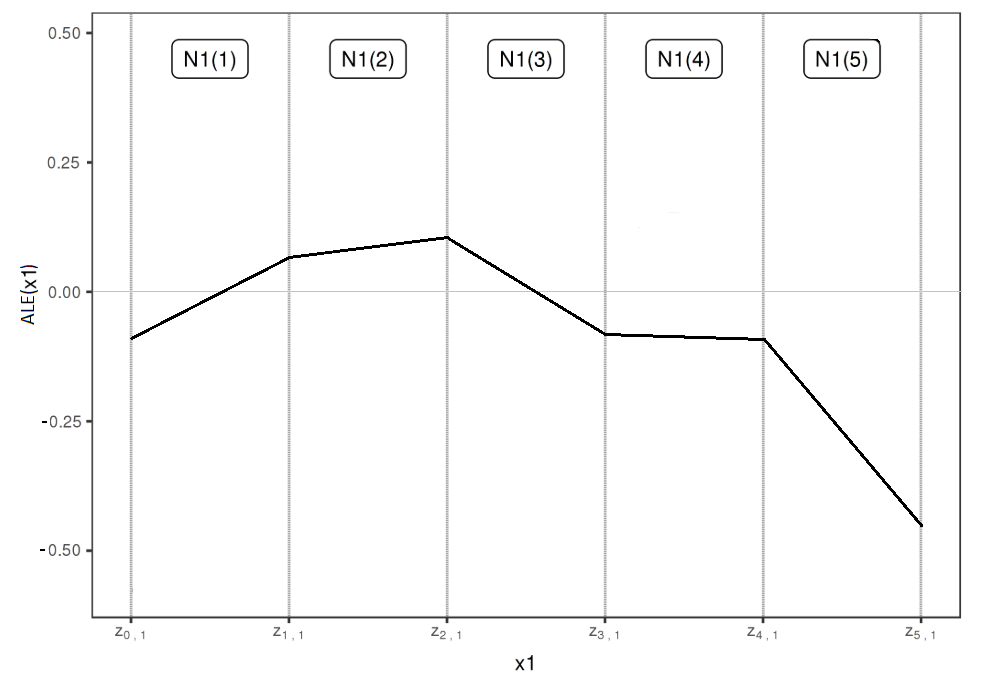
\includegraphics[width=13.75in]{images/ale_example} \caption{bla bla interpretation of ALE bla bla}\label{fig:unnamed-chunk-2}
\end{figure}



TODO: interpret it ;-)

Next to this case - one numeric feature of interest - in the next
chapter methods and interpretation for ALE with two numeric features or
one categorical feature will be looked at in detail. Furthermore we will
pay attention to the size of the intervals the data is evaluatet on
which can be crucial for the expressiveness of the ALE in some data and
learner combinations.

\chapter{Permutation Feature Importance and
LOCO}\label{permutation-feature-importance-and-loco}

\section{Permutation Feature
Importance}\label{permutation-feature-importance}

\section{Leave-One-Covariate-Out
(LOCO)}\label{leave-one-covariate-out-loco}

\chapter{Local Interpretable Model-agnostic
Explanations}\label{local-interpretable-model-agnostic-explanations}

\bibliography{book.bib,packages.bib}

\backmatter
\printindex

\end{document}
